\chapter*{Annexe 3: Théorème de Cantor}
\addcontentsline{toc}{chapter}{Annexe 3: Théorème de Cantor}
\noindent Soit $X \subseteq \R^n$, on rappelle les définitions suivantes :

\medskip % Ajoute un petit espace vertical pour aérer

\noindent Soit $a \in \R^n$. On dit que $a$ est un point d'\textbf{accumulation} de $X$ s'il satisfait l'une des propriétés équivalentes~suivantes :
\begin{itemize}[label=\textbullet, nosep, leftmargin=1.5cm, topsep=2pt]
    \item $\forall V \in \voisinage_a, \quad V \cap X \setminus \{a\} \neq \varnothing$
    \item $\exists (x_n)_{n \in I} \subseteq X, \quad (\forall n \in I, \ x_n \neq a) \land (x_n \to a)$
    \item $\forall V \in \voisinage_a, \quad |V \cap X| \ge \aleph_0$
\end{itemize}

\medskip

\noindent Intuitivement, il s'agit d'un point qui peut être approché par d'autres points de $X$. Une notion plus forte encore est possible : on dit que $a$ est un point de \textbf{condensation} si :
\[
\forall V \in \voisinage_a, \quad |V \cap X| > \aleph_0
\]
Pour la suite, on note $X'$ le dérivé de $X$ \ie l'ensemble des points d'accumulation de $X$.

\begin{lemme}
    $X$ est fermé si et seulement si $X'\subseteq X$
\end{lemme}
\begin{proof}
    Supposons que $X$ soit fermé, on sait donc que $X= \operatorname{adh}(X)= \{\lim x_n\in \R^n
    \mid (x_n)\subseteq X\}$. Comme les points d'accumulation sont des points limites de suites de $X$, on a bien $X'\subseteq \operatorname{adh} X = X$. On suppose que $X'\subseteq X$. Soit $(x_n)_{n\in I}$ une suite de $X$ convergeant vers $a\in \R ^n$. On a soit $\forall n\in I \quad x_n\neq a$ alors par hypothèse $a\in X$, soit $\exists n,\ x_n = a$ d'où $a\in X$ vu que $\forall n \in I\quad x_n\in X$. On en déduit que $X$ est fermé. 
\end{proof}

\begin{lemme}
    $X'$ est fermé.
\end{lemme}
\begin{proof}
    Il suffit de montrer que $X''\subseteq  X'$. Soit $a\in X''$. Par définition, il existe $(x_n)_{n\in I}\subseteq X'$ tel que $(x_n)$ converge vers $a$ et tel que $\forall n\in I \quad x_n\neq a$. Comme tous les termes de la suite $(x_n)$ sont des points d'accumulations de $X$, on a
    \[
    \forall n,\:\exists y_n\in \operatorname{B}\left(x_n,1/n\right)\cap X \quad (y_n\neq x_n)\land (y_n\neq a)
    \]
    Ainsi, on obtient l'existence d'une suite $(y_n)_{n\in I}$ de $X$ dont tous les termes sont différents de $a$. Montrons que $(y_n)$ converge vers $a$. Soit $\varepsilon>0$, nous avons que
    \begin{itemize}
        \item $\exists N_1\in \mathbb{N} \quad \forall n\ge N_1 \quad \|x_n-a\|\leq \varepsilon/2 $
        \item $\exists N_2\in \mathbb{N} \quad \forall n\ge N_2 \quad \|x_n-y_n\|\leq 1/n\leq \varepsilon/2$
    \end{itemize}
    En prenant $N_0= \max\{N_1,N_2\}$ et $n\ge N_0$, on obtient facilement que $\|y_n-a\|\le \varepsilon$. D'où le fait que $a\in X'$.
\end{proof}


\tikzset{every picture/.style={line width=0.75pt}} %set default line width to 0.75pt        
\begin{center}
    

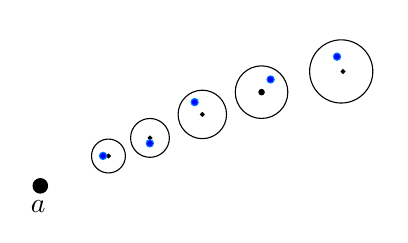
\begin{tikzpicture}[x=0.75pt,y=0.75pt,yscale=-1,xscale=1]
%uncomment if require: \path (0,300); %set diagram left start at 0, and has height of 300

%Shape: Circle [id:dp4438140625397845] 
\draw  [fill={rgb, 255:red, 0; green, 0; blue, 0 }  ,fill opacity=1 ] (121.37,177.44) .. controls (121.31,179.36) and (119.71,180.88) .. (117.79,180.82) .. controls (115.87,180.77) and (114.36,179.17) .. (114.41,177.25) .. controls (114.47,175.33) and (116.07,173.82) .. (117.99,173.87) .. controls (119.91,173.92) and (121.42,175.52) .. (121.37,177.44) -- cycle ;
%Shape: Circle [id:dp4411877441761919] 
\draw  [fill={rgb, 255:red, 0; green, 0; blue, 0 }  ,fill opacity=1 ] (171.6,154.26) .. controls (171.59,154.74) and (171.19,155.12) .. (170.71,155.11) .. controls (170.23,155.1) and (169.85,154.7) .. (169.87,154.22) .. controls (169.88,153.74) and (170.28,153.36) .. (170.76,153.37) .. controls (171.24,153.38) and (171.62,153.78) .. (171.6,154.26) -- cycle ;
%Shape: Circle [id:dp9569406968886757] 
\draw  [fill={rgb, 255:red, 0; green, 0; blue, 0 }  ,fill opacity=1 ] (151.6,162.98) .. controls (151.59,163.46) and (151.2,163.84) .. (150.72,163.83) .. controls (150.24,163.83) and (149.85,163.43) .. (149.86,162.95) .. controls (149.86,162.47) and (150.26,162.09) .. (150.74,162.1) .. controls (151.22,162.1) and (151.6,162.5) .. (151.6,162.98) -- cycle ;
%Shape: Circle [id:dp6199256074403536] 
\draw  [fill={rgb, 255:red, 0; green, 0; blue, 0 }  ,fill opacity=1 ] (196.82,142.95) .. controls (196.8,143.43) and (196.4,143.81) .. (195.93,143.8) .. controls (195.45,143.79) and (195.07,143.39) .. (195.08,142.91) .. controls (195.09,142.43) and (195.49,142.05) .. (195.97,142.06) .. controls (196.45,142.07) and (196.83,142.47) .. (196.82,142.95) -- cycle ;
%Shape: Circle [id:dp9490242719983103] 
\draw  [fill={rgb, 255:red, 0; green, 0; blue, 0 }  ,fill opacity=1 ] (264.6,122.26) .. controls (264.59,122.74) and (264.19,123.12) .. (263.71,123.11) .. controls (263.23,123.1) and (262.85,122.7) .. (262.87,122.22) .. controls (262.88,121.74) and (263.28,121.36) .. (263.76,121.37) .. controls (264.24,121.38) and (264.62,121.78) .. (264.6,122.26) -- cycle ;
%Shape: Circle [id:dp24439689220719696] 
\draw   (247.65,122.22) .. controls (247.65,113.81) and (254.46,106.99) .. (262.87,106.99) .. controls (271.27,106.99) and (278.09,113.81) .. (278.09,122.22) .. controls (278.09,130.62) and (271.27,137.44) .. (262.87,137.44) .. controls (254.46,137.44) and (247.65,130.62) .. (247.65,122.22) -- cycle ;
%Shape: Circle [id:dp7786647322141198] 
\draw   (211.82,132.2) .. controls (211.82,125.2) and (217.49,119.53) .. (224.49,119.53) .. controls (231.48,119.53) and (237.15,125.2) .. (237.15,132.2) .. controls (237.15,139.2) and (231.48,144.87) .. (224.49,144.87) .. controls (217.49,144.87) and (211.82,139.2) .. (211.82,132.2) -- cycle ;
%Shape: Circle [id:dp6744362085498908] 
\draw   (184.28,142.93) .. controls (184.28,136.49) and (189.51,131.26) .. (195.95,131.26) .. controls (202.39,131.26) and (207.62,136.49) .. (207.62,142.93) .. controls (207.62,149.37) and (202.39,154.6) .. (195.95,154.6) .. controls (189.51,154.6) and (184.28,149.37) .. (184.28,142.93) -- cycle ;
%Shape: Circle [id:dp37286062417864596] 
\draw   (161.39,154.24) .. controls (161.39,149.08) and (165.57,144.89) .. (170.74,144.89) .. controls (175.9,144.89) and (180.08,149.08) .. (180.08,154.24) .. controls (180.08,159.4) and (175.9,163.59) .. (170.74,163.59) .. controls (165.57,163.59) and (161.39,159.4) .. (161.39,154.24) -- cycle ;
%Shape: Circle [id:dp10146177458474981] 
\draw   (142.56,162.97) .. controls (142.56,158.46) and (146.22,154.8) .. (150.73,154.8) .. controls (155.24,154.8) and (158.89,158.46) .. (158.89,162.97) .. controls (158.89,167.48) and (155.24,171.13) .. (150.73,171.13) .. controls (146.22,171.13) and (142.56,167.48) .. (142.56,162.97) -- cycle ;
%Shape: Circle [id:dp5204353527064275] 
\draw  [fill={rgb, 255:red, 0; green, 0; blue, 0 }  ,fill opacity=1 ] (225.78,132.24) .. controls (225.76,132.95) and (225.17,133.52) .. (224.45,133.5) .. controls (223.73,133.48) and (223.17,132.88) .. (223.19,132.16) .. controls (223.21,131.45) and (223.81,130.88) .. (224.52,130.9) .. controls (225.24,130.92) and (225.8,131.52) .. (225.78,132.24) -- cycle ;
%Shape: Circle [id:dp19574576919738862] 
\draw  [color={rgb, 255:red, 0; green, 116; blue, 255 }  ,draw opacity=1 ][fill={rgb, 255:red, 2; green, 5; blue, 255 }  ,fill opacity=1 ] (262.58,115.13) .. controls (262.55,116.09) and (261.75,116.85) .. (260.79,116.82) .. controls (259.83,116.8) and (259.08,116) .. (259.1,115.04) .. controls (259.13,114.08) and (259.93,113.32) .. (260.89,113.35) .. controls (261.85,113.37) and (262.61,114.17) .. (262.58,115.13) -- cycle ;
%Shape: Circle [id:dp30920362535162604] 
\draw  [color={rgb, 255:red, 0; green, 116; blue, 255 }  ,draw opacity=1 ][fill={rgb, 255:red, 2; green, 5; blue, 255 }  ,fill opacity=1 ] (230.58,126.13) .. controls (230.55,127.09) and (229.75,127.85) .. (228.79,127.82) .. controls (227.83,127.8) and (227.08,127) .. (227.1,126.04) .. controls (227.13,125.08) and (227.93,124.32) .. (228.89,124.35) .. controls (229.85,124.37) and (230.61,125.17) .. (230.58,126.13) -- cycle ;
%Shape: Circle [id:dp20281146408073158] 
\draw  [color={rgb, 255:red, 0; green, 116; blue, 255 }  ,draw opacity=1 ][fill={rgb, 255:red, 2; green, 5; blue, 255 }  ,fill opacity=1 ] (193.97,137.06) .. controls (193.95,138.02) and (193.15,138.78) .. (192.19,138.75) .. controls (191.23,138.72) and (190.47,137.92) .. (190.5,136.96) .. controls (190.52,136) and (191.32,135.25) .. (192.28,135.27) .. controls (193.24,135.3) and (194,136.1) .. (193.97,137.06) -- cycle ;
%Shape: Circle [id:dp011682685484896704] 
\draw  [color={rgb, 255:red, 0; green, 116; blue, 255 }  ,draw opacity=1 ][fill={rgb, 255:red, 2; green, 5; blue, 255 }  ,fill opacity=1 ] (172.4,156.9) .. controls (172.37,157.86) and (171.57,158.61) .. (170.61,158.59) .. controls (169.65,158.56) and (168.9,157.76) .. (168.93,156.8) .. controls (168.95,155.84) and (169.75,155.08) .. (170.71,155.11) .. controls (171.67,155.14) and (172.43,155.94) .. (172.4,156.9) -- cycle ;
%Shape: Circle [id:dp782211877821206] 
\draw  [color={rgb, 255:red, 0; green, 116; blue, 255 }  ,draw opacity=1 ][fill={rgb, 255:red, 2; green, 5; blue, 255 }  ,fill opacity=1 ] (149.86,162.95) .. controls (149.83,163.91) and (149.03,164.67) .. (148.07,164.64) .. controls (147.11,164.62) and (146.35,163.82) .. (146.38,162.86) .. controls (146.41,161.9) and (147.21,161.14) .. (148.17,161.17) .. controls (149.13,161.19) and (149.88,161.99) .. (149.86,162.95) -- cycle ;

% Text Node
\draw (112.07,183.4) node [anchor=north west][inner sep=0.75pt]    {$a$};
% Text Node
\draw (120.07,152.4) node [anchor=north west][inner sep=0.75pt]    {$\dotsc $};
% Text Node
\draw (279.07,101.4) node [anchor=north west][inner sep=0.75pt]    {$\dotsc $};


\end{tikzpicture}
\end{center}
Ce lemme nous permet d'appréhender un peu mieux comment des points d'un fermé $X$ s'approchent d'un point de $X''$. C'est à dire que pour chaque élément $a$ de $X''$ nous avons au moins une suite $(x_n)$ de $X$ convergeant vers $a$ avec pour chaque $n$ l'existence d'une suite $(y_m)$ de $X$ convergeant vers $x_n$.
\newpage

\noindent Pour illustrer ce phénomène considérons l'ensemble $E= \{\frac{1}{n}+\frac{1}{m}\mid n,m\in \mathbb{N^*\cup \{\infty\}}\}$ en adoptant la convention $\frac{1}{\infty}=0$.
Autrement dit, $E= \{0\}\cup \{\frac1 n\mid n\ge 1 \}\cup \{\frac{1}{n}+\frac1 m \mid n,m\ge 1\}$ et on peut montrer que $E'= \{\frac1n\mid n\ge 1\}$ et $E''=\{0\}$. Les détails sont laissés au lecteur. On a alors que , ici, pour $0\in E''$ on a la suite $(\frac 1 n)$ de $E$ et converge vers $a$ et pour chaque terme de la suite pour un $n_0$ fixé, on a la suite $(\frac{1}{n_0}+\frac{1}{n})$ de $E$ qui converge vers $\frac{1}{n_0}$. On remarque alors que , intuitivement, dériver successivement $E$ supprime, à chaque étape, les points les plus "extérieurs" de $E$.

\medskip

\noindent Au vu, du lemme précédent il est naturel d'établir la suite des dérivées successives de $E$. On définit la suite des dérivées de $X$, $\left(X^{(\alpha)}\right)$ par récurrence transfinie sur $\alpha$ un ordinal, de la manière suivante.
\begin{itemize}[label=\textbullet, nosep, leftmargin=1.5cm, topsep=2pt]
\item $X^{(0)}=X$
\item $X^{(\alpha+1)}=\left(X^{(\alpha)}\right)'$ pour $\alpha$ un ordinal successeur.
\item $X^{(\lambda)}= \bigcap_{\beta<\lambda}X^{(\beta)}$ pour $\lambda$ un ordinal limite.
\end{itemize}
Constatons les conséquences directes des lemmes précédents.

\begin{lemme}
    Pour tout ordinal $\alpha \ge 1 $, $X^{(\alpha)}$ est fermé. Autrement dit, $X^{(\alpha)}\supseteq X^{(\alpha +1)}$.
\end{lemme}

\begin{proof}
Procédons par récurrence transfinie sur l'ordinal $\alpha \ge 1$ :
\begin{itemize}[label=\textbullet]
    \item \textbf{Initialisation ($\alpha = 1$) :} D'après les lemmes 1 et 2, l'ensemble dérivé $X^{(1)} = X'$ est fermé. Puisqu'un ensemble fermé contient par définition tous ses points d'accumulation, on a immédiatement $X^{(2)} = (X^{(1)})' \subseteq X^{(1)}$.
    
    \item \textbf{Hérédité} (Cas successeur) : Supposons que $X^{(\alpha)}$ soit fermé pour un ordinal $\alpha$. Par définition, $X^{(\alpha+1)} = (X^{(\alpha)})'$. D'après le lemme 2, l'ensemble dérivé d'un ensemble quelconque est fermé, donc $X^{(\alpha+1)}$ est fermé. De plus, l'hypothèse de fermeture sur $X^{(\alpha)}$ implique l'inclusion $X^{(\alpha+1)} \subseteq X^{(\alpha)}$.
    
    \item \textbf{Cas limite :} Soit $\lambda$ un ordinal limite tel que le résultat est vrai pour tout $\beta < \lambda$. On définit $X^{(\lambda)} = \bigcap_{\beta < \lambda} X^{(\beta)}$. En tant qu'intersection d'une famille d'ensembles fermés, $X^{(\lambda)}$ est lui-même fermé. 
\end{itemize}
Par principe de récurrence transfinie, le lemme est démontré pour tout ordinal $\alpha \ge 1$.
\end{proof}


\noindent Nous allons donc nous intéresser à la suite des dérivées d'un fermé $X$. Vu ce qui précède, cette suite est décroissante au sens de l'inclusion.

\[
X\supseteq X'\supseteq \dots \supseteq X^{(n)}\supseteq \dots \supseteq X^{(\omega)}\supseteq \dots \supseteq X^{(\alpha)}\supseteq \dots
\]
\medskip

\noindent On dit que la suite $X^{(\alpha)}$ se \textbf{stabilise}  s'il existe $\gamma$ un ordinal tel que $X^{(\gamma)}= X^{(\gamma+1)}$. Notons que les ordinaux étant des b.o., il existe un plus petit ordinal ayant cette propriété disons $\beta$. On dit alors que la suite se stabilise en $\beta$.

\medskip

\noindent On pourrait se questionner quant à la nécessité d'utiliser les ordinaux pour indicer notre suite plutôt que les naturels. Étudions alors un exemple d'une suite qui se stabilise mais pas à une étape strictement avant $\omega$. Avant cela, notons qu'il est facile de construire un ensemble qui se stabilise à un naturel $k+1$. On construit un tel ensemble $A_k$ de manière similaire à l'exemple précédent. On définit $$A_k=\left\{\sum_{i=1}^k\frac{1}{n_i}\mid n_i\in \mathbb{N}^*\cup\{\infty\}\right\}\subseteq [0,k]$$
On peut montrer par récurrence (en adoptant les conventions usuels)
\[
\forall \ell \leq k \quad A^{(\ell)}_k=A_{k-\ell}
\]
On a alors $A^{(k)}_k= \{0\}$ et donc $A_k^{(k+1)}= \varnothing$.
\newpage
\noindent On remarque également que l'ensemble $E$ de notre exemple est $A_2$. Notre interprétation de $A_2$, donné plutôt, s'étend à n'importe quel $A_k$ qu'on peut donc voir comme une nuage de point.

\medskip

\begin{center} % On remplace figure par center pour éviter que ça "flotte"
    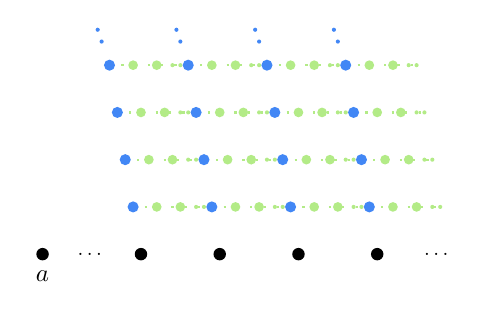
\begin{tikzpicture}[scale=0.5, every node/.style={transform shape}] % Scale réduit à 0.5
        
        % Définition des couleurs
        \definecolor{colA2}{RGB}{66, 135, 245}   
        \definecolor{colA3}{RGB}{179, 235, 135}  

        % Point limite a
        \fill[black] (0, 0) circle (4.5pt) node[below, scale=1.8, yshift=-3pt] {$a$};
        \node[scale=1.5] at (1.2, 0) {$\dots$}; 

        % Boucles
        \foreach \x in {2.5, 4.5, 6.5, 8.5} {
            \fill[black] (\x, 0) circle (4.5pt);

            \foreach \dy/\dx in {1.2/-0.2, 2.4/-0.4, 3.6/-0.6, 4.8/-0.8} {
                \fill[colA2] (\x+\dx, \dy) circle (4pt);

                % Accumulation vers la droite (A3)
                \draw[colA3, loosely dotted, thick] (\x+\dx+0.3, \dy) -- (\x+\dx+1.8, \dy);
                \fill[colA3] (\x+\dx+0.6, \dy) circle (3.5pt);
                \fill[colA3] (\x+\dx+1.2, \dy) circle (3.5pt);
                \fill[colA3] (\x+\dx+1.6, \dy) circle (1.5pt);
                \fill[colA3] (\x+\dx+1.8, \dy) circle (1.5pt);
            }
            % Accumulation vers le haut (A2)
            \fill[colA2] (\x-1.0, 5.4) circle (1.5pt);
            \fill[colA2] (\x-1.1, 5.7) circle (1.5pt);
        }
        \node[scale=1.5] at (10.0, 0) {$\dots$};

    \end{tikzpicture}
    %\captionof{figure}{Représentation locale de $A_3$} % Nécessite \usepackage{capt-of} ou \usepackage{caption}
\end{center}

Grâce aux ensembles $A_k$, on peut construire l'ensemble $B$ tel que la suite $B^{(\alpha)}$ se stabilise en $\omega+1$. On définit $ = \frac{1}{2^k}+ \frac{1}{k2^{k+2}}A_k$, les ensembles $B_k$ sont donc le résultat d'une homothétie de rapport $\frac{1}{k2^{k+2}}$ suivie d'une translation de $\frac{1}{2^k}$ de $A_k$. L'idée ici, est de faire en sorte que les $B_k$ ne se chevauchent pas les un les autres.
Pour atteindre l'ordinal $\omega$, nous juxtaposons donc ces blocs $A_k$ en les isolant par des transformations affines. On définit :
\[
B=\{0\}\cup \bigcup_{k=1}^{\infty}B_k
\]
On peut effectivement vérifier que les $B_k$ sont disjoints puisque pour tout $k\ge 1$, $B_k\subseteq I_k$ où $I_k := [2^{-k},2^{-k}+2^{-(k+2)}]$ et que nous pouvons facilement vérifier que les éléments de la famille $(I_k)$ sont disjoints deux à deux. Grâce à cela, $B$ est un compact par le théorème de Borel-Lebesgue c'est à dire qu'il s'agit d'un ensemble fermé et borné. Par se fait et la formule suivante ( qui se montre par récurrence) :

\[
\forall n\in \mathbb{N} \quad B^{(n)}=\{0\} \cup \bigcup_{k=1}^{\infty}B_k^{(n)}
\]

On peut remarquer que $B^{(\omega)}= \{0\}$ et que la suite $B^{(\alpha)}$ se stabilise en $\omega+1$ et pas avant. D'où l'intérêt de ne pas considérer que des indices naturels pour étudier la stabilisation la suite des dérivées d'un ensemble. Pour continuer l'étude de cette suite $X^{(\alpha)}$ nous avons besoins d'un théorème fort utile que nous allons démontrer.

\begin{theoreme}
    Tout ensemble $X\subseteq \R^n$ infini non dénombrable admet un point de condensation.
\end{theoreme}

\begin{proof}
    Procédons par l'absurde, on suppose alors que $X$ n'admet aucun point d'accumulation, on suppose donc que $\forall a\in X, \exists V\in \mathcal{V}_a\quad |V\cap X|\leq \aleph_0$. Ce qui est équivalent à $\forall a\in X, \exists r_a\in \R^{>0}\quad |B(a,r_a)\cap X|\leq \aleph_0$. De cette hypothèse, nous obtenons que la famille $(B(a,r_a))_{a\in X}$ recouvre $X$. Cependant nous avons vu que $\R^n$ est à base dénombrable. C'est à dire que tout boule ouverte est une union au plus dénombrable de boule à centre rationnel et de rayon dans $\mathbb{Q}^{>0}$. Il en vient que
    \[
    \forall a\in X, \exists r_a\in \R^{>0},  \exists q_a\in \mathbb Q, \exists r_q\in \mathbb{Q^{>0}} \quad a\in B(q_a,r_q)\subseteq B(a,r_a)
    \]
    On note $I$ l'ensemble de tels $q_a$. On a alors que $(B(q_a,r_q))_{q_a\in I}$ est un recouvrement de $X$. Ainsi,

    \[
    X= \bigcup_{q\in I}B(q,r_q)\cap X
    \]
    Clairement $\forall q_a\in I, |B(q_a,r_q)\cap X|\leq \aleph_0$ car $B(q_a,r_q)\cap X\subseteq B(a,r_a)\cap X$. De plus, $I$ est au plus dénombrable car $\mathbb Q$ l'est. $X$ étant une union au plus dénombrable d'ensemble au plus dénombrable, il est au plus dénombrable, par les résultats sur les cardinaux. Ce qui est absurde.
\end{proof}
\noindent Désormais supposons $X$ fermé,

\begin{lemme}
    L'ensemble $X\setminus X '$ est au plus dénombrable.
\end{lemme}

\begin{proof}
Si ce n'était pas le cas, on aurait que
\[
\Cond(X\setminus X')\cap X\setminus X'\neq \varnothing
\]
Ce qui nous mènerait à $X'\cap X\setminus X'\neq \varnothing$
\end{proof}
De ce lemme, on déduit que quelque soit l'ordinal $\alpha$ nous avons $|X^{(\alpha)}\setminus X^{(\alpha+1)}|\le \aleph_0$. Autrement dit le nombres de points enlevés à chaque étape de la dérivation est au plus dénombrable. Un exemple tel que $X\setminus X'$ soit dénombrable est simplement $A_1$. Pour la suite, on note $\omega_1$ le plus petit ordinal infini non dénombrable. Par définition il s'agit de $\aleph_1$ cependant on distinguera ici ces deux notations pour éviter toutes ambiguïté quant aux opérations qu'on pourrait effectuer sur ces derniers.

\begin{lemme}
   Soit $\alpha <\omega_1$ $X\setminus X^{(\alpha)}$ est au plus dénombrable.
\end{lemme}

\begin{proof}
    Cela vient du fait que $X\setminus X^{(\alpha)}= \bigcup_{\beta<\alpha}X^{(\beta)}\setminus X^{(\beta+1)}$.
\end{proof}
Autrement dit, après toute étape au plus dénombrable nous n'avons enlevé qu'au plus un nombre dénombrable de point. De plus, on remarque que si la suite n'est pas stationnaire avant $\omega_1$ alors $X\setminus X^{\omega_1}$ n'est pas dénombrable car à chaque étape nous avons enlevé au moins un point et qu'il y a un nombre non dénombrable d'étape. Par le théorème $1$, $X\setminus X^{(\omega_1)}$ admet un point de condensation.
 \begin{lemme}
        Soit $(X_n)_{n\in\N}$ une suite décroissante de fermés non-vides telles que $\operatorname{diam}(X_n)\to 0$. Alors $\bigcap_{n\in\N} X_n $ est un singleton.
\end{lemme}
\begin{proof}
Nous avons:
\begin{description}
    \item[Unicité : ] Soient, par l'absurde, $x\ne y \in\bigcap_{n\in\N} X_n$. Prenons $N_1,N_2\in\N$ tel que $x\in X_{N_1}$ et $y\in X_{N_2}$. Avec $N:=2\cdot\lceil\max(\norm{x-y}^{-1}, N_1,N_2)\rceil$, on a $x,y\in X_N$ mais $\norm{x-y}<\operatorname{diam} X_N$, c'est absurde. 
    \item[Existence : ] Puisque les $X_n$ sont non vides, on peut prendre une suite $(x_n)_{n\in\N}\subseteq X_0$ telle que $\forall n,\ x_n\in X_n$. Montrons que cette suite est de Cauchy. Soit $\varepsilon>0$. Par convergence du diamètre des $X_n$, il existe $N$ tel que $\operatorname{diam} X_n<\varepsilon$. On a alors, par décroissance des $X_n$, $(x_n)_{n\ge N}\subseteq X_N$.On en déduit que $(x_n)_{n\in\N}$ est de Cauchy.
    Donc $x = \lim x_n$ existe. De plus, on a que, pour tout $n^*\in\N$, $x = \lim_{n\ge n^*} x_n\in X_{n^*}$ par fermeture. Donc $x\in \bigcap_{n\in\N} X_n $.
\end{description}
\end{proof}
\begin{theoreme}
    Si $X$ est parfait et non vide (c'est à dire que $X=X'$) alors $|X|= 2^{\aleph_0}$ et $X= \operatorname{Cond(X)}$.
\end{theoreme}

\begin{proof}
Soit $a\in X$ et $V\in\mathscr V_a$.
 Nous allons montrer qu'il existe une injection $\varphi : \{0,1\}^{\mathbb N}\to X\cap V$.
 
On appelle mot de longueur $n$ une application $w : [\![1,n]\!]\to \{0,1\}$. Par récurrence sur $n$ la longueur, on définit les boules fermées $B_w$ associées à un mot $w$ de la façon suivante :
\begin{description}
    \item[Initialisation : ] On prend $B_{\varnothing} = \overline{B(a,\varepsilon_{\varnothing})}$ de sorte que $B_{\varnothing}\subseteq V$.
    \item[Pas de récurrence : ] Soit $B_w = \overline{B(a_w,\varepsilon_w)}$ avec $a_w\in X$ et $w$ un mot de longueur $n$. Par hypothèse, $\abs{\overline{B(a_w,\varepsilon_<)}}\ge\aleph_0\ge 3$. On peut donc y prendre $a_{w0}\ne a_{w1}$ différents de $a_w$. Posons $$\varepsilon_{w0}:=\varepsilon_{w1}:=\min\left(\frac{1}{n+1}, \frac{\varepsilon}{2}, \frac{\norm{a_{w0} - a_{w1}}}{3}\right)$$ afin que $\forall w, B_w\subseteq B_{w0},B_{w1}, B_{w0}\cap B_{w1} = \varnothing$ et, si $n\ge 1$, $\operatorname{diam}(B_w)\le \frac 2n$.
    Soit $f\in \{0,1\}^{\N}$. On pose $\varphi(f)$ l'unique élément de $\bigcap_{n\in\N}B_{f_{\mid[\![1,n]\!]}}\cap X$. Par le lemme, cet élément existe et est unique. Montrons maintenant que $\varphi$ est injective. Soient $f_1\ne f_2$. Soit $i$ le plus petit indice tel que $f_1(i)\ne f_2(i)$. On a alors $B_{f_{1\mid[\![1,i]\!]}}\cap B_{f_{2\mid[\![1,i]\!]}} = \varnothing$ d'où $\varphi(f_1)\ne\varphi(f_2)$.
Dès lors, par existence de $\varphi$, il vient que $\forall a\in X, \forall V\in\mathscr V _a, \abs{X\cap V}\ge 2^{\aleph_0}>\aleph_0$. Donc $X\subseteq\Cond(X)$. Or $\Cond(X)\subseteq X' = X$. De plus, il existe $a\in X$, et $\R_n$ est un voisinage de tous ses points. Donc $2^{\aleph_0}\le \abs{X\cap \R^n} = \abs{X}\le \abs{\R^n} = 2^{\aleph_0}$.
\end{description}
  
\end{proof}

\begin{center}
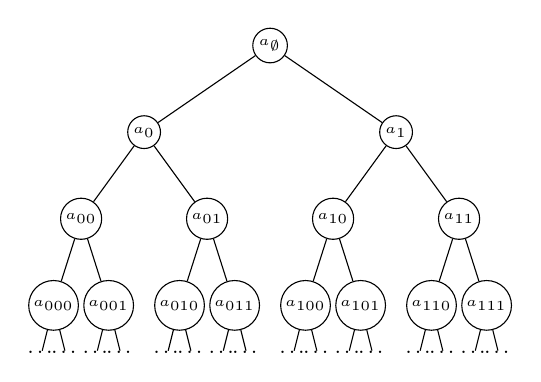
\begin{tikzpicture}[
    % Espacements principaux de l'arbre
    level 1/.style={sibling distance=3.2cm, level distance=1.1cm},
    level 2/.style={sibling distance=1.6cm, level distance=1.1cm},
    level 3/.style={sibling distance=0.7cm, level distance=1.1cm}, % Plus serré pour les groupes
    % Espacements pour les branches finales (niveau 4)
    level 4/.style={sibling distance=0.3cm, level distance=0.6cm},
    % Style pour les nœuds avec indices (cercles)
    idxnode/.style={circle, draw=black, fill=white, inner sep=1.2pt, font=\tiny, thin},
    % Style pour les points de continuation (sans bordure)
    dotsnode/.style={draw=none, fill=none, inner sep=0pt, font=\tiny\bf},
    % Style pour les lignes de liaison
    edge from parent/.style={draw, thin}
]

% Racine
\node[idxnode] (root) {$a_{\emptyset}$}
    child {
        node[idxnode] {$a_0$}
        child {
            node[idxnode] {$a_{00}$}
            child {node[idxnode] {$a_{000}$}
                child {node[dotsnode] {\dots}} % Branche gauche (continuation 0)
                child {node[dotsnode] {\dots}} % Branche droite (continuation 1)
            }
            child {node[idxnode] {$a_{001}$}
                child {node[dotsnode] {\dots}}
                child {node[dotsnode] {\dots}}
            }
        }
        child {
            node[idxnode] {$a_{01}$}
            child {node[idxnode] {$a_{010}$}
                child {node[dotsnode] {\dots}}
                child {node[dotsnode] {\dots}}
            }
            child {node[idxnode] {$a_{011}$}
                child {node[dotsnode] {\dots}}
                child {node[dotsnode] {\dots}}
            }
        }
    }
    child {
        node[idxnode] {$a_1$}
        child {
            node[idxnode] {$a_{10}$}
            child {node[idxnode] {$a_{100}$}
                child {node[dotsnode] {\dots}}
                child {node[dotsnode] {\dots}}
            }
            child {node[idxnode] {$a_{101}$}
                child {node[dotsnode] {\dots}}
                child {node[dotsnode] {\dots}}
            }
        }
        child {
            node[idxnode] {$a_{11}$}
            child {node[idxnode] {$a_{110}$}
                child {node[dotsnode] {\dots}}
                child {node[dotsnode] {\dots}}
            }
            child {node[idxnode] {$a_{111}$}
                child {node[dotsnode] {\dots}}
                child {node[dotsnode] {\dots}}
            }
        }
    };

\end{tikzpicture}
\end{center}

Ainsi, si la suite se stabilise en un ordinal $\beta$ alors alors soit $X^{(\beta)}= \varnothing$, soit $X^{(\beta)}$ contient $2^{\aleph_0}$ points. Par conséquent, on déduit que si $X$ est fermé et tel que la suite des dérivées se stabilise en $\beta$ tel que $X^{(\beta)}\neq \varnothing$ alors $|X|= 2^{\aleph_0}$ puisque $X= X^{(\beta)}\cup X\setminus X^{(\beta)}$. A présent, Nous allons faire une disjonction de cas. Etudions les deux cas possibles : Soit $\operatorname{Cond}(X)= \varnothing$, soit $\operatorname{Cond}(X)\neq \varnothing$.\par
\medskip
\noindent Dans le premier cas, si $\operatorname{Cond}(X)= \varnothing $ alors par le théorème $1$, la suite se stabilise forcément en un $\beta <\omega_1$. De plus, toujours par ce dernier théorème, on aura $X^{(\beta)}= \varnothing$. On va maintenant examiner le cas où $\operatorname{Cond}(X)$ est non vide.

\begin{lemme}
    Soit $Y\subseteq X$, si $Y$ est parfait alors pour tout ordinal $\alpha$, $Y\subseteq X^{(\alpha)}$.
\end{lemme}

\begin{proof}
    Il est clair que toute suite de points de $Y$ est une suite de point de $X$ donc $Y'\subseteq X'$. On procède alors par récurrence transfinie.
    \begin{itemize}[label=\textbullet]
    \item \textbf{Initialisation ($\alpha = 0$) :}. On a par définition $Y\subseteq X$.
    
    \item \textbf{Hérédité} (Cas successeur) : Supposons que $X^{(\alpha)}$ contienne $Y$ pour un ordinal $\alpha$. Vu ce qui précède, $Y'\subseteq X^{(\alpha+1)}= (X^{(\alpha)})'$. Comme $Y$ est parfait on a bien $Y\subseteq  X^{(\alpha+1)}$.
    
    \item \textbf{Cas limite :} Soit $\lambda$ un ordinal limite tel que le résultat est vrai pour tout $\beta < \lambda$. On a $X^{(\lambda)} = \bigcap_{\beta < \lambda} X^{(\beta)}$. En tant qu'intersection d'ensemble contenant $Y$, $Y\subseteq X^{(\lambda)}$. 
\end{itemize}
\end{proof}
Un ensemble sous ensemble parfait de $X$ ne peut donc pas être éliminé par la dérivation. Intuitivement, un tel ensemble est trop dense et ne contient aucun point "extérieur" qui puisse être enlevé. Le lemme suivant est donc tout naturel.

\begin{lemme}
    $\operatorname{Cond}(X)$ est parfait.
\end{lemme}

\begin{proof}
    La démonstration s'effectue par double inclusion.

    \noindent 1. Montrons que $(\Cond(X))' \subseteq \Cond(X)$ : \\
    Soit $a$ un point limite de $\Cond(X)$. Puisque $X$ est fermé et que $\Cond(X) \subset X$. Soit $V$ un voisinage ouvert de $A$. Nous avons donc
    \[
    V\cap \Cond(X) \neq \varnothing
    \]
    Donc il existe un certain $b_V \in \Cond(X)\cap V$. Comme $V$ est ouvert il est voisinage de tous ses points et en particulier $b_V$ qui est un point de condensation de $X$ donc 
    \[|V\cap X|>\aleph_0\]
    d'où le fait que $a\in \Cond(X)$
    \vspace{0.3cm}
    \noindent 2. Montrons que $\Cond(X) \subseteq (\Cond(X))'$ : \\
    Soit $a \in \Cond(X)$. Montrons que tout voisinage $V$ de $a$ contient un point $b_V \in \Cond(X)$ distinct de $a$, ce qui prouvera que $a$ est un point limite de $\Cond(X)$. 
    Le voisinage $V$ contient, par définition, un nombre non dénombrable de points de $X$ distincts de $a$. 
    D'après le théorème, tout ensemble non dénombrable contient au moins un de ses propres points de condensation. Ainsi, $V$ contient un point de $\Cond(X)$ autre que $a$. 
    On a donc $a \in (\Cond(X))'$, ce qui prouve la densité en soi de l'ensemble.
\end{proof}

\begin{theoreme}
    Soit $X\subseteq \R^n$ un ensemble fermé, si pour un ordinal $\alpha$ $X^{(\alpha)}=X^{(\alpha+1)}$ alors $X^{(\alpha)}= \Cond(X)$. De plus, la suite des dérivées de $X$ se stabilise en un ordinal au plus dénombrable.
\end{theoreme}

\begin{proof}
    Si $\Cond (X)$ est vide alors on a déjà établi que dans ce cas la suite $X^{(\alpha)}$ se stabilise en un ordinal $\beta<\omega_1$ et tel que $X^{(\beta)}=\varnothing=\Cond (X)$. Et si $\Cond (X)$ est non vide alors par les deux lemmes précédents pour tout  ordinal $\alpha$, on a $\Cond(X)\subseteq X^{(\alpha)}$. Donc la suite se stabilise en un $\beta< \omega_1$ car sinon comme vu précédemment $X\setminus X^{(\omega_1)}$ admettrait un point d'accumulation. On aurait donc $\Cond(X)\cap(X\setminus \Cond(X))\neq \varnothing$ ce qui est absurde. De plus, $X^{(\beta)}$ est parfait donc $X^{(\beta)}=\Cond(X^{(\beta)})\subseteq \Cond(X)$ et l'autre inclusion provient du lemme précédent.
\end{proof}

Autrement dit, on vient de montrer que la suite $X^{(\alpha)}$ fini forcément par se stabiliser et que le noyau dure de l'ensemble est l'ensemble de ses points de condensation.  

\begin{theoreme}[Cantor-Bendixon]
    Tout ensemble fermé $X \subseteq \mathbb{R}^n$ est soit fini soit dénombrable, soit de cardinalité $2^{\aleph_0}$. 
\end{theoreme}
\begin{proof}
 Par le théorème précédent on sait que la suite $X^{(\alpha)}$ se stabilise en un $\beta < \omega_1$ tel que $X^{(\beta)}= \Cond (X)$. On sait également que
 \[
 X= \Cond(X)\sqcup X\setminus X^{(\beta)}
 \]
 De là, clairement si $\Cond (X)$ est vide alors $X$ est au plus dénombrable. Dans le cas où $\Cond(X)$ est non vide $X$ est une union entre un ensemble de cardinalité $2^{\aleph _0}$ et d'un ensemble au plus dénombrable donc $X$ est de cardinal $2^{\aleph_0}$.
\end{proof}
En fait, on peut découper $X$ comme une union disjointe entre son noyau (sa partie parfaite) et les autres points plus "espacés". Une analogie pertinente pour comprendre les fermés dans $\R^{n}$ est de les voir comme des ognons que nous pellons.
En effet, à chaque étape nous enlevons un couche de l’oignon mais se processus ne peut pas continuer indéfiniment puisque à un moment soit nous auront enlevé toutes les couches de l'oignon (il ne reste plus rien), ce qui correspond au cas où $\Cond (X)$ est vide. Soit on arrive sur un noyau trop dense pour être pellé, ce qui cette foi correspond au cas où $\Cond (X)$ est non vide. Dans les deux cas on comprend mieux la structure de l'oignon et donc on peut en déduire sa taille. Cela est dû au fait que lorsqu'on pelle l'oignon on enlève qu'un nombre de point au plus dénombrable. 